%%%%%%%%%%%%%%%%%%%%%%%%%%%%%%%%%%%%%%%%%%%%%%%%%%%%%%%%%%%%%%%%%%%%%%%%%%%%%
%% Original default rstudio/pandoc latex file
%% upated by @jhollist 09/15/2014
%% inspired by @cboetting https://github.com/cboettig/template and
%% @rmflight blog posts:
%% http://rmflight.github.io/posts/2014/07/analyses_as_packages.html 
%% http://rmflight.github.io/posts/2014/07/vignetteAnalysis.html).  
%%%%%%%%%%%%%%%%%%%%%%%%%%%%%%%%%%%%%%%%%%%%%%%%%%%%%%%%%%%%%%%%%%%%%%%%%%%%%

\documentclass[11pt,]{article}
\usepackage[T1]{fontenc}
\usepackage{lmodern}
\usepackage{amssymb,amsmath}
\usepackage{ifxetex,ifluatex}
\usepackage{fixltx2e} % provides \textsubscript
% use upquote if available, for straight quotes in verbatim environments
\IfFileExists{upquote.sty}{\usepackage{upquote}}{}
\ifnum 0\ifxetex 1\fi\ifluatex 1\fi=0 % if pdftex
  \usepackage[utf8]{inputenc}
\else % if luatex or xelatex
  \ifxetex
    \usepackage{mathspec}
    \usepackage{xltxtra,xunicode}
  \else
    \usepackage{fontspec}
  \fi
  \defaultfontfeatures{Mapping=tex-text,Scale=MatchLowercase}
  \newcommand{\euro}{€}
\fi
% use microtype if available
\IfFileExists{microtype.sty}{\usepackage{microtype}}{}
\usepackage[margin=1in]{geometry}
\usepackage{graphicx}
% Redefine \includegraphics so that, unless explicit options are
% given, the image width will not exceed the width of the page.
% Images get their normal width if they fit onto the page, but
% are scaled down if they would overflow the margins.
\makeatletter
\def\ScaleIfNeeded{%
  \ifdim\Gin@nat@width>\linewidth
    \linewidth
  \else
    \Gin@nat@width
  \fi
}
\makeatother
\let\Oldincludegraphics\includegraphics
{%
 \catcode`\@=11\relax%
 \gdef\includegraphics{\@ifnextchar[{\Oldincludegraphics}{\Oldincludegraphics[width=\ScaleIfNeeded]}}%
}%
\ifxetex
  \usepackage[setpagesize=false, % page size defined by xetex
              unicode=false, % unicode breaks when used with xetex
              xetex]{hyperref}
\else
  \usepackage[unicode=true]{hyperref}
\fi
\hypersetup{breaklinks=true,
            bookmarks=true,
            pdfauthor={},
            pdftitle={Combined effects of protein expression variance and correlation on multicomponent systems},
            colorlinks=true,
            citecolor=blue,
            urlcolor=blue,
            linkcolor=magenta,
            pdfborder={0 0 0}}
\urlstyle{same}  % don't use monospace font for urls
\setlength{\parindent}{0pt}
\setlength{\parskip}{6pt plus 2pt minus 1pt}
\setlength{\emergencystretch}{3em}  % prevent overfull lines
\setcounter{secnumdepth}{0}

%%%%%%%%%%%%%%%%%%%%%%%%%%%%%%%%%%%%%%%%%%%%%%%%%%%%%%%%
%Changes borrowed from @cboettig, added by @jhollist 
% A modified page layout 
\textwidth 6.75in
\oddsidemargin -0.15in
\evensidemargin -0.15in
\textheight 9in
\topmargin -0.5in
\usepackage{lineno} % add 
%%%%%%%%%%%%%%%%%%%%%%%%%%%%%%%%%%%%%%%%%%%%%%%%%%%%%%%%

%%%%%%%%%%%%%%%%%%%%%%%%%%%%%%%%%%%%%%%%%%%%%%%%%%%%%%%%
%%Packages and layout changes by @jhollist 09/15/2014
\usepackage{ragged2e}
\usepackage[font=normalsize]{caption}
  \usepackage[doublespacing]{setspace}
\usepackage{parskip}
\usepackage{fancyhdr}
\pagestyle{fancy}
\fancyhf{}
\renewcommand{\headrulewidth}{0pt}
\lfoot{\thepage}
%%Changed default abstract width and added lines
\renewenvironment{abstract}{
  \hfill\begin{minipage}{1\textwidth}
  \rule{\textwidth}{1pt}\vspace{5pt}
  \normalsize
  \begin{justify}
  \bfseries\abstractname\vspace{5pt}
  \end{justify}}
  {\par\noindent\rule{\textwidth}{1pt}\end{minipage}
}
%%%%%%%%%%%%%%%%%%%%%%%%%%%%%%%%%%%%%%%%%%%%%%%%%%%%%%%%

\title{Combined effects of protein expression variance and correlation on
multicomponent systems}
\author{
Kyle M. Kovary
Mary N. Teruel
}
\date{}
% Allowing for landscape pages
\usepackage{lscape}
\newcommand{\blandscape}{\begin{landscape}}
\newcommand{\elandscape}{\end{landscape}}

% Left justification of the text: see https://www.sharelatex.com/learn/Text_alignment
% \usepackage[document]{ragged2e} % already in the latex template
\newcommand{\bleft}{\begin{flushleft}}
\newcommand{\eleft}{\end{flushleft}}
\usepackage{float} \floatplacement{figure}{H} \newcommand{\beginsupplement}{\setcounter{table}{0}  \renewcommand{\thetable}{S\arabic{table}} \setcounter{figure}{0} \renewcommand{\thefigure}{S\arabic{figure}}}

%%Fix tightlist error: https://stackoverflow.com/questions/40438037/tightlist-error-using-pandoc-with-markdown
%%Added 2018-03-26 
\providecommand{\tightlist}{%
  \setlength{\itemsep}{0pt}\setlength{\parskip}{0pt}}
%%%  
  

\begin{document}
%%Edited by @jhollist 09/15/2014
%%Adds title from YAML
\begin{singlespace}
\begin{center}
\huge Combined effects of protein expression variance and correlation on
multicomponent systems
\end{center}
%%Adds Author, correspond email asterisk, and affilnum from YAML
\begin{center}
\large
Kyle M. Kovary \textsuperscript{1} 
Mary N. Teruel \textsuperscript{1} 
\end{center}
%%Adds affiliations from YAML
\begin{justify}
\footnotesize \emph{ 
\\*
\textsuperscript{1}Department of Chemical and Systems Biology, Stanford University,
Stanford, CA 94305, USA.\\*
}
%%Adds corresponding author email(s) from YAML
\newcounter{num}
\setcounter{num}{1}
\\[0.1cm]
\footnotesize \emph{ 
}
\end{justify}
%%Adds date from YAML
\normalsize

\begin{abstract}
Protein expression variation leads to phenotypic variance between cells.
This has been demonstrated in cell signaling and differentiation
decisions. Additionally coordinated expression of proteins between cells
can tune signaling pathways either towards a more binary or analog
modality. Though there is some evidence in bulk cell measurements and in
bacteria that certain heteromeric subunits or metabolic pathways may be
expressed in a coordinated fashion (i.e.~operons in bacteria), there has
not been a direct measurement of coordinated expression of proteins
(independent of TFs) in metazoans (vertebrates?). Here, we measure
cell-to-cell variability of relative protein abundance using
quantitative proteomics of individual \emph{Xenopus laevis} eggs and
show that proteins involved in metabolic pathways or members of
heteromeric complexes tend to have high correlations with other members
of those pathways/complexes. Our previous work highlighted the fact that
correlated expression increases the total variation of a pathway, so one
would reason that certain pathways or complexes would need to compensate
of this extra source of by reducing the variation of expression of these
pathways or complexes. To test this we computed total variance score
that took into account both the coefficient of variance and correlations
between proteins in a pathway and found that the lower 10\% of GO terms
were highly enriched for metabolic pathways. When we looked at the
relationship between CV and R between these GO terms we found a negative
relationship between them, demonstrating that increased correlation
needs to come at the expense of decreased variance. Simple molecular
models of heteromeric complexes and metabolic pathways demonstrate that
this tradeoff can result in higher efficiencies in both function and
reduced energy waste. Together, our study argues for a control principle
whereby coordinated expression of proteins in a pathway can require
lower variance in order to reduce the overall pathway variance, enabling
accurate control of active complexes or metabolic pathway activity.
\end{abstract}
\end{singlespace}


\emph{Keywords}: single cell, proteomics, stochasticity

\doublespace

\bleft

\justify

\hypertarget{introduction}{%
\section{Introduction}\label{introduction}}

The coordinated expression of proteins is vital for cellular function,
from maintaining a dynamic steady state to differentiation of cells into
specialized types and tissues. This coordinated regulation of protein
abundance is subject to stochastic expression levels, and modules
(pathways, complexes, etc.) have varying tolerances of noise for proper
function ranging from precise stoichiometric coordination, to high
levels of noise that can result in heterogeneous responses of
homogeneous cell populations to identical stimuli (Suderman et al.,
2017). The ability to regulate coordinated expression has been
demonstrated to occur via transcription (transcription factors,
chromatin regulation), translation (specialized ribosomes, mRNA
structure/modifications), and degradation (E3 ligases), all of which are
subject to stochastic expression and interactions. This noise has been
shown be utilized by cells for bet hedging strategies as well as tissue
size maintenance (more concrete examples to come). Additionally, the
combination of variability and coordinated expression (correlation) of
proteins can lead to increased population level control in binary
decisions, and a decreased ability to execute analog signaling (Kovary
et al., 2018; Suderman et al., 2017).

There have been numerous studies, both targeted and unbiased, of
coordinated protein expression or expression variation independently
that have shown the important impacts of these parameters on cellular
function. However, both of these parameters (variation and correlation)
act together to determine the total variance of a system. To
systematically assess these properties of single cells at a large scale,
we conducted shotgun proteomics analyses on \emph{Xenopus laevis} eggs
during their first cell cycle. We have found this model to be ideal at
this nascent stage of the single cell proteomics field because of their
large size and tractability. An advantage of this approach is that we
can get around much of the signal to noise issues that accompany
studying single cells caused by low sample protein levels. Additionally,
at this stage of development transcription is restricted, allowing for
insights into non-transcriptional control of protein expression. By
utilizing isobaric tagging and shotgun mass spectrometry we were able to
measure \textgreater{}1000 proteins across 25 single cells in 5 mass
spectrometry runs.

With this data set we have been able to, for the first time, gain
insights into the relationship between protein expression variance,
coordinated protein expression, and total variance within modules at a
proteomic scale in single cells. We identified classes of proteins that
include heteromeric complexes and metabolic pathways that are expressed
in such a way that the increase in total variance of the system caused
by high coordinated expression of proteins is offset by decreased
variation, allowing for modules that rely on stoichiometric expression
and low level of variance to maintain a low level of total system
variance. By counter balancing coordinated expression (correlation) of
proteins in a module with low expression variance, cells are able to
decrease the total variance of a given complex or pathway. This elegant
balancing act may allow for finer control of metabolic throughput and
controlling the number of potentially formed complexes though
stoichiometric control.

\hypertarget{results}{%
\section{Results}\label{results}}

\hypertarget{single-cell-proteomics-reveals-global-protein-expression-variability-and-coordinated-expression-between-protein-pairs.}{%
\subsection{Single cell proteomics reveals global protein expression
variability and coordinated expression between protein
pairs.}\label{single-cell-proteomics-reveals-global-protein-expression-variability-and-coordinated-expression-between-protein-pairs.}}

The specific requirements for coordinated protein expression of pathways
or complexes can vary, with some requiring strict stoichiometric
regulation and others having much more relaxed requirements. Strict
stoichiometry scenarios require coordinated expression of proteins
(Figure 1A, top), and others can have uncoordinated expression (Figure
1A bottom). At the single cell level, coordinated expression will result
in a high correlation coefficient, whereas un-coordinated expression
will result in a low correlation coefficient (Figure 1B). Even when the
expression variation (standard deviation or coefficient of variation)
and abundance is identical between these two scenarios, the total
variance of a pathway or complex can be significantly different due to
the variance sum law:
\(var\left(\sum_{i=1}^n X_{i}\right) = \sum_{i=1}^{n} var(X_{i}) + 2\sum_{i,j:i<j}^{n} cov(X_{i},X_{j})\)
(Figure 1C). Our previous work has shown that this effect is important
in single cell pathway activation dynamics (Kovary et al., 2018).

In order to study the relationship between protein expression variance
and co-expression (correlated expression) of cellular pathways and
complexes at the proteome level, we utilized \emph{Xenopus laevis} eggs
as a single cell model. Activated \emph{Xenopus laevis} eggs were
collected at 5 time points across the first cell cycle (0, 20, 40, 60,
and 80 minutes), with 5 eggs at each time point (Fig 1D). Using TMT
multiplexing and mass spectrometry, we were able to determine the
relative abundance of more than 1300 proteins in single cells.
Expression of these proteins across the time course of the cell cycle
showed no dynamic patterns, revealing that these highly expressed
proteins are likely not regulated by cell cycle processes. Additionally,
a PCA analysis of these eggs showed no discernible clustering on cell
cycle time (Fig S2).

To determine the expression variability for the measured proteins
between single cells, we calculated the variance and coefficient of
variation (CV) across all samples. This showed a wide range of variation
containing multiple distributions (Fig 1E), many of which are consistent
with our previous study of variation using targeted mass spectrometry
(Fig S2). An added benefit to measuring these proteins in parallel is
that we are able to calculate coordinated expression of protein pairs at
single cell resolution. Using the Pearson correlation coefficient, we
were able to determine the coordinated expression of nearly 2 million
protein pairs (Fig 1F-G). The distribution of correlation coefficients
fit a normal distribution centered around 0, with the majority of
protein pairs appearing to not show significant co-regulation. However,
there appear to be a significant number of protein pairs containing high
correlation coefficients, and a clustered heat map shows that many
highly co-regulated pairs cluster together (Fig 1G).

\hypertarget{variance-sum-law-reveals-modules-that-utilize-a-trade-off-between-protein-co-expression-and-noise}{%
\subsection{Variance sum law reveals modules that utilize a trade-off
between protein co-expression and
noise}\label{variance-sum-law-reveals-modules-that-utilize-a-trade-off-between-protein-co-expression-and-noise}}

Multicomponent modules such as heteromeric protein complexes and
metabolic and signaling pathways have a certain tolerance for noise. Two
components of the noise of these systems are the expression variance of
the individual proteins, as well as the correlation or co-variance of
expression between the proteins. This means that if a group of proteins
have a positive correlation, then the total variance will be higher than
if there was no correlation. This single cell proteomics data set gave
us an excellent opportunity to see how variance and co-expression of
proteins are related in low variance and high variance modules. The
total variance of a module can be calculated using the variance sum law,
where for a group of proteins \(X_{1},\dotsc,X_{n}\), the total variance
of the group is:
\[\sigma_{{}_{total}}^2 = \sum_{i=1}^{n} \sigma_{X_{i}}^2 + 2\sum_{i,j:i<j}^{n} \rho(X_{i},X_{j})\sigma_{X_i}\sigma_{X_j}\]

To categorize the measured protein expression data into modules, we
utilized GO term and KEGG pathway annotations. Since pathways and
complexes have varying numbers of proteins, and the number of proteins
in a module is highly influential on the total variance sum, we
normalized the total variance sum by the number of components (Fig. xA
and xB) to eliminate this confounding dependency. With the normalized
total variance metric, we could separate modules into high and low
variance categories (Fig 2A). Since co-expression of proteins (positive
correlation between protein expression) increases the total variance, we
expected to see the high variance modules to be enriched for high levels
of both protein expression variance and co-expression (Fig 1B and 1C,
red). However, we were surprised to see that the low variance modules
were also enriched for high levels of co-expression of proteins, with
some of the mean correlation coefficients of modules as high as those in
the high variance category (Fig 1B, orange shaded region).

We wondered how these protein modules dealt with the increased variance
load caused by the high numbers of correlated proteins, so we looked at
the pairwise relationship between the mean variance of the modules and
the mean correlation coefficients (Fig 2D and S1). The low variance
modules uniquely showed a significant negative correlation (R = 0.49)
between these two metrics, showing that for modules that enforce a low
level of total variance, co-expression of proteins within that module is
offset by lower expression variance.

\hypertarget{enforcement-of-a-trade-off-between-protein-co-expression-and-noise-increases-efficiency-of-heteromeric-protein-complexes-and-metabolic-pathways}{%
\subsection{Enforcement of a trade-off between protein co-expression and
noise increases efficiency of heteromeric protein complexes and
metabolic
pathways}\label{enforcement-of-a-trade-off-between-protein-co-expression-and-noise-increases-efficiency-of-heteromeric-protein-complexes-and-metabolic-pathways}}

Interestingly, we saw the low total variance and high coordinated
expression sub population contained many metabolic pathways as well as
multisubunit complexes, while the high total variance and high
coordinated expression sub-population contained many signalling pathways
(Fig. 2D, Fig. 3E-H). Previous studies have shown that protein complex
components are produced stoichiometricly (Taggart and Li, 2018) across
eukaryotic species and that co-expression of pathway specific enzymes
are tightly regulated post-transcriptionally across species
(Jean-Beno\emph{Lalanne and James C. Taggart and Monica S. Guo and Lydia
Herzel and Ariel Schieler and Gene-Wei Li}, 2018). This led us to
wondered what the implications were for the synergy of maintaing low
total variance with high levels of co-expression of the members of
protein complexes and metabolic pathways.

To test why complexes observed in our data set and others, (i.e.~core
members of the ribosome (Fig 4A)), coordinate co-expression and
expression variation, we imagined an idealized 10 member heteromeric
complex (Fig 4B). Coordinated expression could allow for tight control
of the total number of assembled complexes. However, this on it's own is
not sufficient since high levels of individual protein variance would
result in an increased number of partially assembled complexes. In this
idealized complex, we titrated the correlation coefficients between all
10 members along with the individual expression variation and saw that
increased correlations and decreasing variance had a synergistic effect
in allowing for the control of the total number of fully assembled
complexes (Fig 4C.). Additionally, there is a large regime with high
correlations and low variation that allow for low total variance of the
system.

We also observed a number of metabolic pathways that had similar
variation and correlation properties as the protein complexes, such as
the pentose phosphate pathway and glycolysis. Both of these pathways
have a large number of reversible enzymes. For a reversible enzymatic
pathway, the concentrations of the enzymes dictate the rate of the
reaction, and the concentrations of the reaction products relative to
the substrates can dictate the direction of the reaction equilibrium.
Therefore, strict balance of the concentration of enzymes using low
levels of variance and strict control of the relative abundances of the
enzymes is a potentially important step in regulating metabolic pathway
output. To test this hypothesis, we constructed an idealized metabolic
model (or a physiological model??) and tested the ability of the pathway
to maximize output (Fig 5x). (haven't done this, would like feedback /
help).

\hypertarget{discussion}{%
\subsection{Discussion}\label{discussion}}

\newpage

\hypertarget{figures}{%
\section{Figures}\label{figures}}

\begin{figure}
\centering
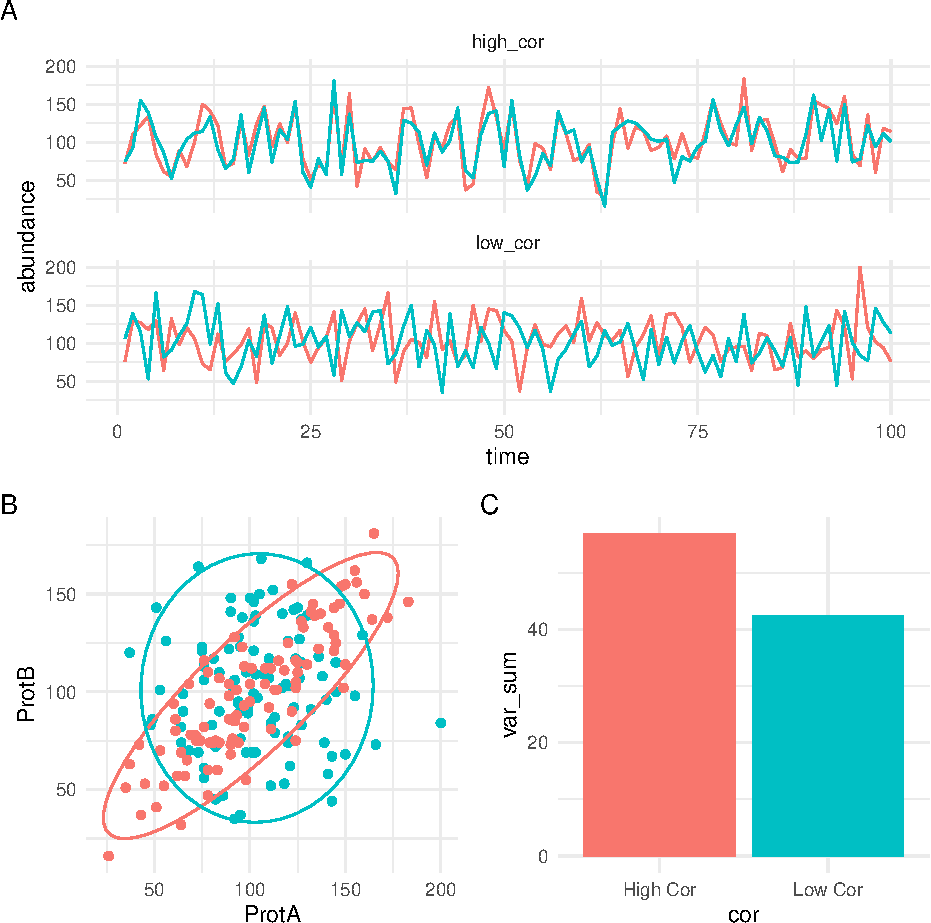
\includegraphics{output/figures/figure_1-1.pdf}
\caption{A) Simulated expression of two proteins over time in a single
cell with a mean of 100 and a standard deviation of 30 with expression
correlations of 0 and 0.8. B) Pairwise plots of the two proteins in the
single cells between uncorrelated and correlated scenarios. C) The total
variance between the uncorrelated and correlated scenarios from A and B.
D) To measure protein expression variance and coordinated expression, 25
eggs at 5 time points during the first cell cycle were analyzed with
multiplexed shotgun mass spectrometry. E) Histogram of the coefficient
of variation of all measured proteins. F) Histogram of the pairwise
correlation coefficients between all measured proteins. G) Heat-map of
the pairwise correlation coefficients between all measured protein
pairs.}
\end{figure}

\newpage

\begin{figure}
\centering
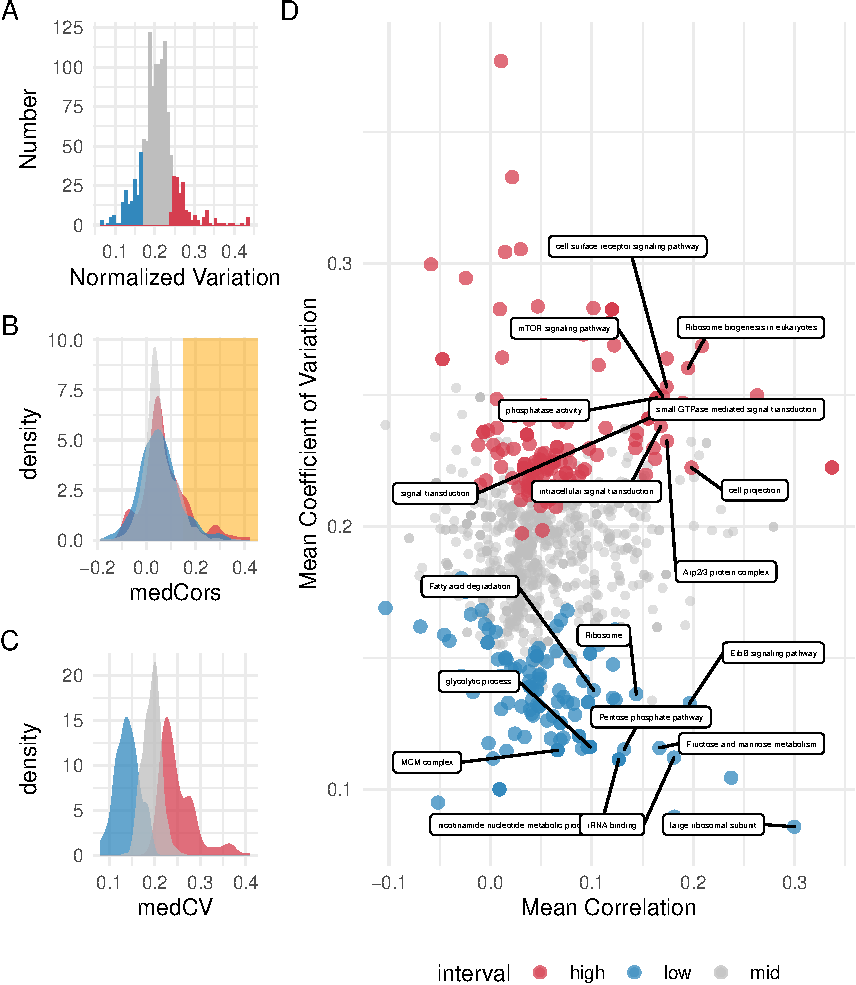
\includegraphics{output/figures/figure_2-1.pdf}
\caption{A) Histogram of the normalized variation values across all of
the GO terms and KEGG pathways. The bottom and top \textasciitilde{}15\%
are colored blue and red respectively. B) Distributions of the mean
correlation coefficient across all groups of proteins. Both the top and
bottom 15\% of normalized variation groups had peaks of high levels of
mean correlation coefficients. C) Distributions of the mean coefficient
of variation across all groups of proteins. The top and bottom
\textasciitilde{}15\% of normalized variation groups were largely
separated. D) Pairwise plot between the mean correlation and mean
coefficient of variation within each GO term and KEGG pathway with color
coding from A. Interestingly, both the top and bottom 10\% of normalized
variation have groups of proteins with high levels of correlation,
despite high correlation adding to total variance. In the lowest 10\% of
normalized variation groups there appears to be a negative correlation
between mean correlation and variation.}
\end{figure}

\newpage

\begin{figure}
\centering
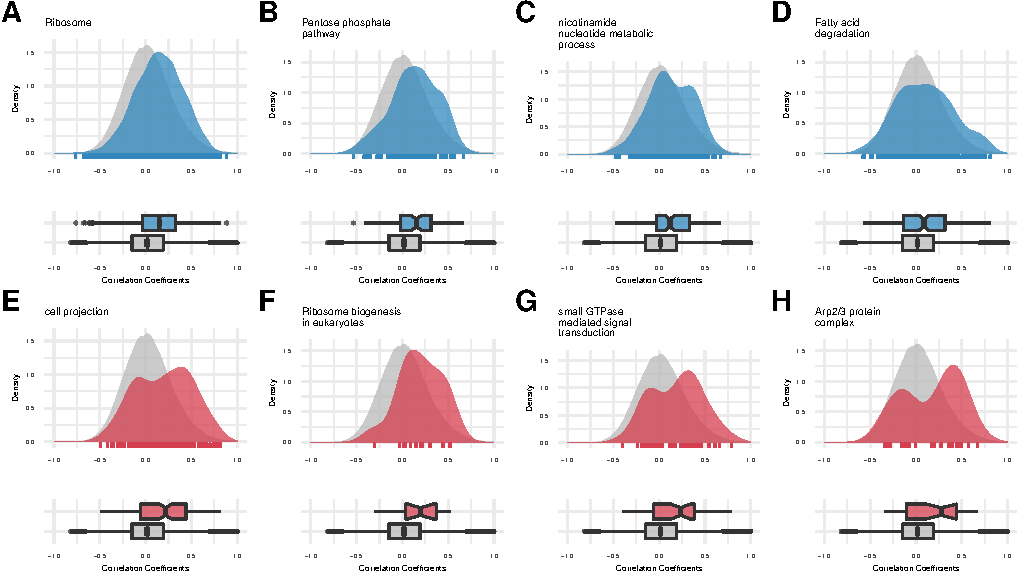
\includegraphics{output/figures/figure_3-1.pdf}
\caption{Density plots of correlation coefficients select protein groups
color coded by low (blue) and high (red) normalized protein variance,
with the distribution of all measured correlation coefficients colored
in grey (rug plot to show the measured correlations coefficients shown
on plot). Below each density plot is a box plot.}
\end{figure}

\newpage

\begin{figure}
\centering
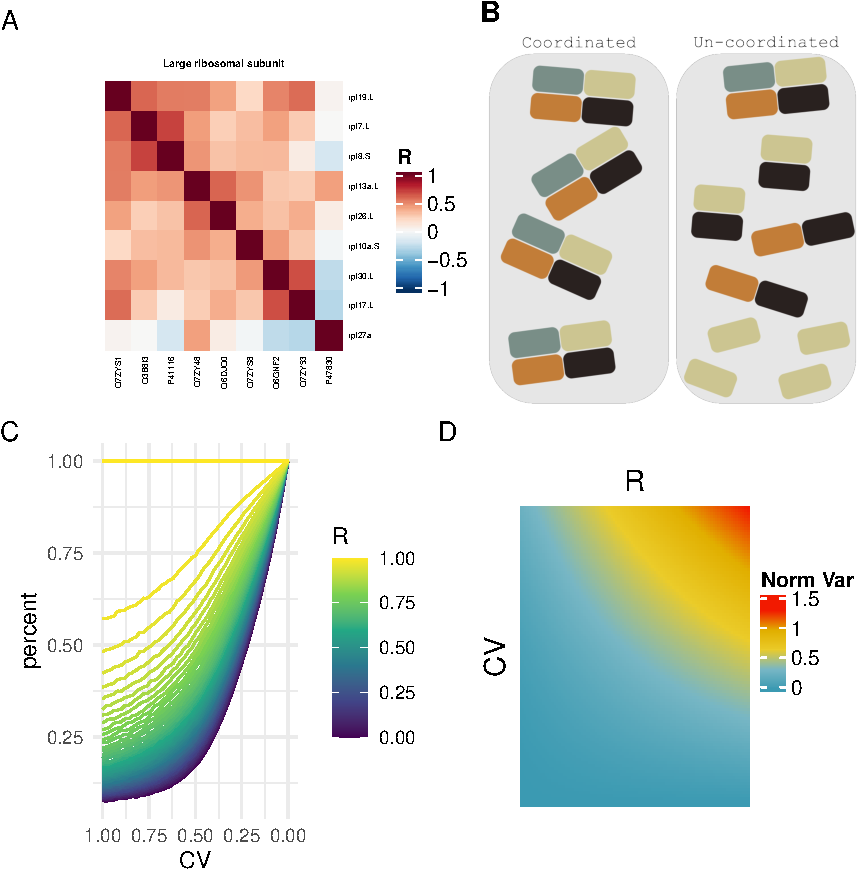
\includegraphics{output/figures/figure_4-1.pdf}
\caption{A) A representative heat-map of one of the low normalized
variation groups with high levels of correlated proteins (Large
ribosomal subunit). B) A simple model showing the percent of potentially
assembled subunits of an idealized heteromeric 10 subunit complex. Both
the variation of expression between the subunits as well as the
coordinated expression between them can effect the percent of maximum
assembled complexes. C) Heat-map showing the total variance as a
function of coefficient of variation and correlation from the idealized
model in B).}
\end{figure}

\newpage

\hypertarget{supplementary-material}{%
\section*{Supplementary material}\label{supplementary-material}}
\addcontentsline{toc}{section}{Supplementary material}

\setcounter{table}{0}  \renewcommand{\thetable}{S\arabic{table}} \setcounter{figure}{0} \renewcommand{\thefigure}{S\arabic{figure}}

\begin{figure}
\centering
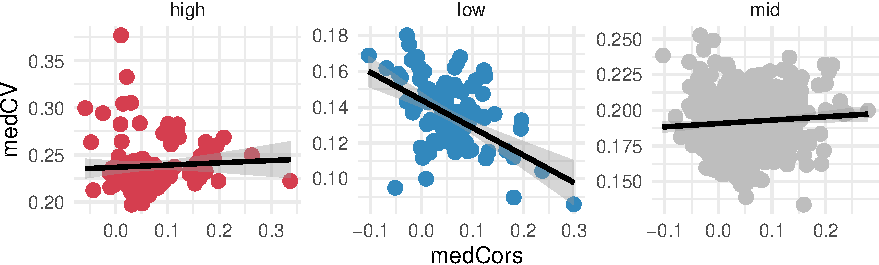
\includegraphics{output/figures/sup_fig_1-1.pdf}
\caption{Pairwise plots of the mean correlation coefficient and mean
coefficient of variation of protein groups with linear fit. The low
variance protein groups have a significant negative correlation between
these two variables, showing that for protein modules that require low
variance and high co-expression, showing that these two
parameters\ldots{} R (high, low, med) = (0.057, -0.485, 0.071)}
\end{figure}

\newpage

\hypertarget{methods}{%
\section{Methods}\label{methods}}

\hypertarget{collection-and-activation-of-xenopus-laevis-eggs}{%
\subsection{Collection and activation of Xenopus laevis
eggs:}\label{collection-and-activation-of-xenopus-laevis-eggs}}

Xenopus egg extracts were prepared based on modifications of a previous
protocol (Tsai et al., 2014). All of the animal protocols used in this
manuscript were approved by the Stanford University Administrative Panel
on Laboratory Animal Care. To induce egg laying, female Xenopus laevis
were injected with human chorionic gonadotropin injection the night
before each experiment. To collect the eggs, the frogs were subjected to
pelvic massage, and the eggs were collected in 1X Marc's Modified
Ringer's (MMR) buffer (0.1 M NaCl, 2 mM KCl, 1 mM MgCl2, 2 mM CaCl2, 5
mM HEPES, pH 7.8). To remove the jelly coat from the eggs, they were
placed in a solution of 2\% cysteine in 1× MMR buffer for 4 min and
gently agitated, after which they were washed four times with 1× MMR
buffer. To activate the cell cycle, eggs were placed in a solution of
0.5 \(\mu\)g/ml of calcium ionophore A23187 (Sigma) and 1X MMR buffer
for 3 min, after which they were washed four times with 1× MMR buffer.
Single eggs were collected at their respective time-points and placed
into 600uL tubes and snap frozen in liquid nitrogen before being stored
at 80°C.

\hypertarget{sample-preparation-for-mass-spectrometry}{%
\subsection{Sample preparation for mass
spectrometry:}\label{sample-preparation-for-mass-spectrometry}}

Single eggs were lysed mechanically by pipetting the egg in 100\(\mu\)L
of lysis buffer (100 mM NaCl, 25 mM Tris pH 8.2, Complete EDTA- free
protease inhibitor cocktail (Sigma). The lysate was then placed in a 400
uLnatural polyethylene micro-centrifuge tube (E\&K Scientific \#485050)
and spun at 15,000 g in a right angle centrifuge (Beckman Microfuge E)
at 4°C for 5 min. The lipid layer was removed by using a razor blade to
cut the tube off just beneath it, and the cytoplasmic fraction was
pipetted into a 1.5-ml protein LoBind tube (Fisher Scientific
\#13-698-794), being careful to leave the yolk behind. To precipitate
the proteins from the cytoplasmic fraction, 1 ml of ice cold acetone was
added to each sample and placed at 20°C overnight. To collect
precipitated proteins, the samples were centrifuged at 18,000 g for 20
min at 4°C. Acetone was decanted, and the protein pellets were
resolubilized in 25\(\mu\)L of 8 M urea. To fully solubilize the protein
pellet, the samples were placed in a shaker for 1 h at room temperature.
The samples were then diluted to 2 M urea with 50 mM ammonium
bicarbonate to a 100\(\mu\)L volume, after which protein concentration
was measured in duplicate with a BCA assay by taking two 10\(\mu\)L
aliquots of each sample. The proteins in the remaining 80\(\mu\)L of
sample volume were reduced with 10 mM TCEP and incubated for 30 min at
37°C, then alkylated with 15 mM iodoacetamide and incubated in the dark
at room temperature.

Next, the samples were diluted to 1 M urea with 50 mM ammonium
bicarbonate. Trypsin (Promega \#V5113) was then added at a ratio of 10
ng trypsin per 1ug protein (no \textless{} 500 ng was added to a
sample). The trypsin digestion was carried out at 37°C for 12--16 h. To
stop the trypsin, formic acid (Fisher \#A117-50) was added at a ratio of
3\(\mu\)l per 100\(\mu\)l of sample to bring the pH down to \textless{}
3.

Peptides were cleaned up using an Oasis HLB uElution plate (Waters),
equilibrated, and washed with 0.04\% trifluoroacetic acid in water, and
eluted in 80\% acetonitrile with 0.2\% formic acid. All solutions used
are HPLC grade. Samples were then lyophilized. To remove any variance
produced by phosphorylated peptides, the samples were
phosphatase-treated. Peptides were resolubilized in 50\(\mu\)L of 1X
NEBuffer 3 (no BSA), and calf intestinal alkaline phosphatase (NEB
\#M0290S) was added at a ratio 0.25 units per lg of peptide and
incubated for 1 h at 37°C. The peptides were cleaned up again according
to steps described above. Peptides were resolubilized in 2\%
acetonitrile and 0.1\% formic acid before MS analysis.

\hypertarget{mass-spectrometry-data-collection}{%
\subsection{Mass spectrometry data
collection:}\label{mass-spectrometry-data-collection}}

Ask SUMS for details

\hypertarget{mass-spectrometry-data-analysis}{%
\subsection{Mass spectrometry data
analysis:}\label{mass-spectrometry-data-analysis}}

Ask SUMS for details

\hypertarget{data-processing}{%
\subsection{Data processing:}\label{data-processing}}

To minimize the effects of non-biological variance, a correction factor
was used to correct for these biases. First, each peptide was normalized
by the median across all of the samples. Second, the vector of all
peptides for each cell was divided by the median value across all
peptides. Before peptides were used to estimate protein abundance,
highly variable peptides needed to be filtered out. Peptides were
grouped by their master UniProt accession number, and all peptides whose
log transformed values were more than 2\(\sigma\) away from the mean
were discarded. Next, protein abundances were estimated by taking the
median normalized value for each peptide for a protein in each sample.
Missing protein levels were imputed using the k-nearest neighbors
algorithm, with k being set to 1 and the similarity measure for distance
the Gower's distance between the proteome vectors.

\clearpage

\hypertarget{references}{%
\section{References}\label{references}}

\hypertarget{refs}{}
\leavevmode\hypertarget{ref-Lalanne_2018}{}%
Jean-Beno\emph{Lalanne and James C. Taggart and Monica S. Guo and Lydia
Herzel and Ariel Schieler and Gene-Wei Li} (2018). Evolutionary
convergence of pathway-specific enzyme expression stoichiometry. Cell
\emph{173}, 749--761.e38.

\leavevmode\hypertarget{ref-Kovary_2018}{}%
Kovary, K.M., Taylor, B., Zhao, M.L., and Teruel, M.N. (2018).
Expression variation and covariation impair analog and enable binary
signaling control. Molecular Systems Biology \emph{14}.

\leavevmode\hypertarget{ref-Suderman_2017}{}%
Suderman, R., Bachman, J.A., Smith, A., Sorger, P.K., and Deeds, E.J.
(2017). Fundamental trade-offs between information flow in single cells
and cellular populations. Proceedings of the National Academy of
Sciences \emph{114}, 5755--5760.

\leavevmode\hypertarget{ref-Taggart_2018}{}%
Taggart, J.C., and Li, G.-W. (2018). Production of protein-complex
components is stoichiometric and lacks general feedback regulation in
eukaryotes. Cell Systems \emph{7}, 580--589.e4.

\leavevmode\hypertarget{ref-Tsai_2014}{}%
Tsai, T.Y.-C., Theriot, J.A., and Ferrell, J.E. (2014). Changes in
oscillatory dynamics in the cell cycle of early xenopus laevis embryos.
PLoS Biology \emph{12}, e1001788.

\eleft

\clearpage

\begin{verbatim}
R version 3.6.1 (2019-07-05)
Platform: x86_64-apple-darwin15.6.0 (64-bit)
Running under: macOS Catalina 10.15.3

Matrix products: default
BLAS:   /Library/Frameworks/R.framework/Versions/3.6/Resources/lib/libRblas.0.dylib
LAPACK: /Library/Frameworks/R.framework/Versions/3.6/Resources/lib/libRlapack.dylib

locale:
[1] en_US.UTF-8/en_US.UTF-8/en_US.UTF-8/C/en_US.UTF-8/en_US.UTF-8

attached base packages:
 [1] parallel  stats4    grid      stats     graphics  grDevices utils    
 [8] datasets  methods   base     

other attached packages:
 [1] circlize_0.4.8       pheatmap_1.0.12      magick_2.3          
 [4] KEGG.db_3.2.3        latex2exp_0.4.0      ggplotify_0.0.4     
 [7] knitcitations_1.0.10 mvtnorm_1.1-0        patchwork_1.0.0     
[10] cowplot_1.0.0        plotly_4.9.2         ggrepel_0.8.1       
[13] GO.db_3.10.0         org.Xl.eg.db_3.10.0  AnnotationDbi_1.48.0
[16] IRanges_2.20.2       S4Vectors_0.24.3     Biobase_2.46.0      
[19] BiocGenerics_0.32.0  VIM_5.1.0            data.table_1.12.8   
[22] colorspace_1.4-1     GGally_1.4.0         ComplexHeatmap_2.2.0
[25] RColorBrewer_1.1-2   forcats_0.5.0        stringr_1.4.0       
[28] dplyr_0.8.5          purrr_0.3.3          readr_1.3.1         
[31] tidyr_1.0.2          tibble_2.1.3         ggplot2_3.3.0.9000  
[34] tidyverse_1.3.0      knitr_1.28          

loaded via a namespace (and not attached):
  [1] readxl_1.3.1        backports_1.1.5     Hmisc_4.3-1        
  [4] plyr_1.8.5          lazyeval_0.2.2      splines_3.6.1      
  [7] sp_1.4-1            digest_0.6.25       htmltools_0.4.0    
 [10] wesanderson_0.3.6   fansi_0.4.1         checkmate_2.0.0    
 [13] magrittr_1.5        memoise_1.1.0       cluster_2.1.0      
 [16] openxlsx_4.1.4      modelr_0.1.6        jpeg_0.1-8.1       
 [19] blob_1.2.1          rvest_0.3.5         haven_2.2.0        
 [22] xfun_0.12           crayon_1.3.4        jsonlite_1.6.1     
 [25] survival_3.1-8      zoo_1.8-7           glue_1.3.1         
 [28] gtable_0.3.0        GetoptLong_0.1.8    car_3.0-6          
 [31] shape_1.4.4         DEoptimR_1.0-8      abind_1.4-5        
 [34] scales_1.1.0        DBI_1.1.0           bibtex_0.4.2.2     
 [37] Rcpp_1.0.3          htmlTable_1.13.3    viridisLite_0.3.0  
 [40] laeken_0.5.1        clue_0.3-57         gridGraphics_0.5-0 
 [43] foreign_0.8-75      bit_1.1-15.2        Formula_1.2-3      
 [46] rsvg_1.3            vcd_1.4-5           htmlwidgets_1.5.1  
 [49] httr_1.4.1          acepack_1.4.1       ellipsis_0.3.0     
 [52] pkgconfig_2.0.3     reshape_0.8.8       farver_2.0.3       
 [55] nnet_7.3-13         dbplyr_1.4.2        tidyselect_1.0.0   
 [58] labeling_0.3        rlang_0.4.4         munsell_0.5.0      
 [61] cellranger_1.1.0    tools_3.6.1         cli_2.0.2          
 [64] generics_0.0.2      RSQLite_2.2.0       ranger_0.12.1      
 [67] broom_0.5.5         evaluate_0.14       yaml_2.2.1         
 [70] RefManageR_1.2.12   bit64_0.9-7         fs_1.3.1           
 [73] zip_2.0.4           robustbase_0.93-5   nlme_3.1-144       
 [76] formatR_1.7         xml2_1.2.2          compiler_3.6.1     
 [79] rstudioapi_0.11     curl_4.3            png_0.1-7          
 [82] e1071_1.7-3         reprex_0.3.0        stringi_1.4.6      
 [85] highr_0.8           lattice_0.20-40     Matrix_1.2-18      
 [88] vctrs_0.2.3         pillar_1.4.3        lifecycle_0.1.0    
 [91] BiocManager_1.30.10 lmtest_0.9-37       GlobalOptions_0.1.1
 [94] latticeExtra_0.6-29 R6_2.4.1            gridExtra_2.3      
 [97] rio_0.5.16          codetools_0.2-16    boot_1.3-24        
[100] MASS_7.3-51.5       assertthat_0.2.1    rjson_0.2.20       
[103] withr_2.1.2         mgcv_1.8-31         hms_0.5.3          
[106] rpart_4.1-15        class_7.3-15        rmarkdown_2.1      
[109] rvcheck_0.1.8       carData_3.0-3       base64enc_0.1-3    
[112] lubridate_1.7.4    
\end{verbatim}

\end{document}